%% Template for EU deliverable, using the deliverable.sty style file

\documentclass[12pt,a4paper,twoside]{report}

%% common package
\usepackage[headers]{deliverable}
\usepackage{xspace}
\usepackage{verbatim}
\usepackage[usenames]{color}
\usepackage[usenames,dvipsnames]{xcolor}
%\usepackage{graphicx}
\usepackage{url}
\usepackage{array}
\usepackage{graphics} 		% for pdf, bitmapped graphics files
\usepackage{graphicx}
\usepackage{epsfig} 		% for postscript graphics files
\usepackage{epstopdf}
\usepackage{caption}
\usepackage[labelformat=simple]{subcaption}
\renewcommand\thesubfigure{(\alph{subfigure})}
\usepackage{nameref}
\usepackage{multirow}
\usepackage{color}
 \usepackage{pdfpages}
%\usepackage{subfigure}
%%

%%insert here other packages needed by sections
%\usepackage{esint}
\usepackage{amstext}
\usepackage{amsmath}	 	% assumes amsmath package installed
\usepackage{amssymb}  		% assumes amsmath package installed
%\renewcommand\thesubfigure{(\alph{subfigure})}
\usepackage{wrapfig}
\usepackage[]{nomencl}		% nomenclatures
%\usepackage{dsfont}
%%

%%%%%%%%%%%%%%%%%%%%%%%%%%%%%% LyX specific LaTeX commands.

%%%%%%%%%%%%%%%%%%%%%%%%%%%%%%%%%%%%%%%%%%%%%%%%%%%%%%%%%%%%%%%%%%%%%%%%%%%%%%
%%% Titlepage
%%%%%%%%%%%%%%%%%%%%%%%%%%%%%%%%%%%%%%%%%%%%%%%%%%%%%%%%%%%%%%%%%%%%%%%%%%%%%%

% declaration of variables used in style
\deliverableDocnumber{D4.3}
\deliverableTitle{Learning of the prioritization policies.}

\deliverableAuthor{Jan Peters$^{1,2}$ and Elmar Rueckert$^1$}
\deliverableResponsiblePartner{TUDA}
\deliverableAffiliation{% Insert here authors affiliations
 $^1$ Intelligent Autonomous Systems Lab, Technische Universit\"at Darmstadt, 64289 Darmstadt, Germany.
  $^2$ Robot Learning Group, Max-Planck Institute for Intelligent Systems,
	Tuebingen, Germany.
}

\deliverableReviewer{}
\deliverableCoordinator{Jan Peters}
\deliverableActivityNumber{n} %% n=1,..,10
\deliverableActivity{Activity Name}
\deliverableDoctype{Deliverable} %% or Prototype
\deliverableClassification{Public} % or Consortium
\deliverableDistribution{Consortium} %
\deliverableStatus{Draft} % Draft or Final
\deliverableDeliveryDate{28/2/2017}
\deliverableFile{Dxx\_DeliverableName.pdf} % please do not use "-" in the name
\deliverableVersion{1.0}
\deliverableDate{Feb.~28, 2017}
\deliverableYear{2017}
\deliverablePages{\pageref{LastPage}}
\deliverableChangelog{v.0.1 & Feb 07, 2017 & Initial draft %%\\\hline
%%              v.2.0 & Feb 20, 2007 & Final version
}
\deliverableProjectStartingDate{1st March 2013}
\deliverableProjectEndDate{28th February 2017}
\deliverableProjectAcronym{CoDyCo}
\deliverableProjectTitle{Whole-Body Compliant Dynamical Contacts in Cognitive Humanoids}
 \deliverableContractNumber{600716}
 \deliverableProjectCoordinator{Istituto Italiano di Tecnologia}
 \deliverableProjectUrl{www.codyco.eu}
 \deliverableFrameworkProgramme{FP7}
 
 \deliverableWorkpackage{WP4}
 \deliverableEditors{Jan Peters and Elmar Rueckert}
 \deliverableContributors{Ryan Lober, Vincent Padois, Olivier Sigaud, Valerio Modugno, Gerhard Neumann, Elmar Rueckert, Giuseppe Oriolo, Jan Peters, Serena Ivaldi, Alex Paraschos, Ugo Chervet}
 \deliverableReviewers{}
\deliverableAbstract{The scope of the current deliverable is to present the results on the learning of the task prioritization policies. 
}
\deliverableKeywordList{contacts, inverse dynamics model learning, probabilistic movement representations, reinforcement learning}


\def\BibPath{./manuscript}       % location of bibtex-files
%%%%%%%%%%%%%%%%%%%%%%%%%%%%%%%%%%%%%%%%%%%%%%%%%%%%%%%%%%%%%%%%%%%%%%%%%%%%%%
%%% Sections
%%%%%%%%%%%%%%%%%%%%%%%%%%%%%%%%%%%%%%%%%%%%%%%%%%%%%%%%%%%%%%%%%%%%%%%%%%%%%%

%% constants
\newcommand{\botegoCaps}{BOTEGO}
\newcommand{\certhCaps}{CERTH}
\newcommand{\cybionCaps}{CYBION}
\newcommand{\nuigCaps}{NUIG}
\newcommand{\ubitechCaps}{UBITECH}

%%
%%%%%%%%%%%%%%%%%%%%%%%%%%%%%% BEGIN DOCUMENT
\begin{document}

\deliverableMaketitle

%%TODO move to style
\newcolumntype{L}[1]{>{\raggedright\let\newline\\\arraybackslash\hspace{0pt}}m{#1}}
\newcolumntype{C}[1]{>{\centering\let\newline\\\arraybackslash\hspace{0pt}}m{#1}}
\newcolumntype{R}[1]{>{\raggedleft\let\newline\\\arraybackslash\hspace{0pt}}m{#1}}

\textbf{Document Revision History}
\begin{center}
\begin{tabular}{|C{2cm}|C{3cm}|p{5cm}|C{4cm}|}
\hline
\textbf{Version}&\textbf{Date}&\textbf{Description}&\textbf{Author}\\\hline
v. 0.1 & Feb. 07 & Initial Draft & Elmar Rueckert\\\hline
v. 0.2 & Feb. 20 & Draft & Elmar Rueckert\\\hline
v. 1.0 & Feb. 21 & Final & Elmar Rueckert\\\hline
\end{tabular}
\end{center}
 
 \clearpage

\newpage
\renewcommand*\contentsname{Table of Contents}
\renewcommand*\listfigurename{Index of Figures}
\tableofcontents
\newpage
%\listoffigures
%\newpage

%%%%%%%%%%%%%%%%%%%%%%%% Start deliverable content here.

\chapter{Introduction}

This deliverable presents results of task T4.4. In total four articles were presented at international robotics conferences (HUMANOIDS, ICRA and IROS) and two articles are currently under review. Below, we discuss the achievements with respect to the task description from the Technical Annex.

\section{Task description from the Technical Annex.} 
The core element of WP3 is the intelligent combination of prioritized tasks, which allows covering a large
variety of possible scenarios while only requiring a small number of elements. Nevertheless, WP3’s
architecture requires a meaningful prioritization scheme that tells the systems which tasks to activate and
how certain tasks can overrule each other. While it is possible to devise such prioritizations for complex
tasks manually (see, e.g., Sentis et al., 2008), the automatic generation from data is much more desirable.
Hence, in this task, we will investigate how a prioritization can be obtained from observing tasks, similar as
in imitation learning, and how it can be self-improved. The relative importance of the tasks imposed by the
prioritization can be changed during execution by the learned prioritization based on the current context.
First, T4.4 will only help reproduce behavior from WP2 on the iCub but subsequently, it will allow for
generalization to novel situations. Expected task outcomes are the following:
\begin{itemize}
\item Objective 1: A learned importance weighting for elementary tasks; weighting will allows appropriate
combinations to generate solutions for new, more complex scenarios.
\item Objective 2: A learned prioritization policy using both imitation and reinforcement learning (see tasks from
WP2); demonstration and generalization to novel situations.
\end{itemize}

\section{Contributions within the CoDyCo consortium.} We developed learning approaches that avoid task interferences prior to the task execution,  
that can be trained through reinforcement learning from a general task objective and from imitation learning in a probabilistic model. 
\begin{itemize}
 \item To objective 1: At UPMC, efficient whole-body control strategies have been developed that 
avoid interferences of multiple task objectives prior to a task execution. Two articles were published at international conferences and 
are summarized in Chapter~\ref{sec:Ryan}. A detailed description can be found in \textit{Deliverable D3.3}. 
\item To objective 2: In a collaboration, INRIA and TUDA studied the learning of task priority profiles for whole-body control. We optimized the parameters of priority profiles with respect to a general task objective through reinforcement learning~\cite{Modugno_PICRA_2016}. This work is presented in Chapter~\ref{sec:Valerio}.
\newline In a followup study, INRIA investigated different stochastic search implementations for reinforcement learning~\cite{modugno2016learning}. An article on the approach is listed in 
Chapter~\ref{sec:Valerio2}. 
\newline In another study, TUDA investigated how task such priority profiles can be obtained from imitation learning. 
A research article of this study is currently under review~\cite{Paraschos_2017}. In Chapter~\ref{sec:Alex}, we present a draft of this contribution. 
\end{itemize}


\chapter{Multiple Task Learning for Whole-Body Reactive Control (UPMC)}\label{sec:Ryan}

In the following three paragraphs, we summarize the work of Ryan Lober, Vincent Padois and Olivier Sigaud on 
learning the task prioritization of multiple tasks. For a detailed report on these two articles we refer to 
\textit{Deliverable D3.3}.

\paragraph*{Multiple Task Optimization using Dynamical Movement Primitives for Whole-Body Reactive Control.}
Whole-body controllers provide the tools to execute
multiple simultaneous tasks on humanoid robots, but
given the robot’s internal and external constraints, interferences
are often generated which impede task completion. Priorities
can be assigned to each task to manage these interferences,
unfortunately, this is often done at the detriment of one or
more tasks. In this paper we present a novel framework for
defining and optimizing multiple tasks in order to resolve
potential interferences prior to task execution and remove the
need for prioritization. Our framework parameterizes tasks
with Dynamical Movement Primitives, simulates and evaluates
their execution, and optimizes their parameters based on a
general compatibility principle, which is independent of the
robot’s topology, tasks or environment. Two test cases on a
simulation of a humanoid robot are used to demonstrate the
successful optimization of initially interfering tasks using this
framework. 

This work was presented at the international conference on humanoid robots~\cite{lober-HUMANOIDS2014}.

\paragraph*{Variance Modulated Task Prioritization in Whole-Body Control.}
Whole-Body Control methods offer the potential
to execute several tasks on highly redundant robots, such as
humanoids. Unfortunately, task combinations often result in
incompatibilities which generate undesirable behaviors. Prioritization
techniques can prevent tasks from perturbing one
another but often to the detriment of the lower precedence
tasks. For many tasks, static prioritization is not necessary
or even appropriate because tasks can often be achieved in
variable ways, as in reaching. In this paper, we show that such
task variability can be used to modulate task priorities during
execution, to temporarily deviate certain tasks as needed, in
the presence of incompatibilities. We first present a method
for mapping from task variance to task priority and then
provide an approach for computing task variance. Through
three common conflict scenarios, we demonstrate that mapping
from task variance to priorities reactively solves a number of
task incompatibilities.

This work was presented at the international conference on intelligent robots and systems~\cite{lober_IROS2015}.

\paragraph*{Task compatibility optimization.}

Highly redundant robots, such as humanoids, can execute multiple simultaneous tasks allowing them to perform complex whole-body behaviors. Unfortunately, tasks are generally planned without close consideration for the underlying controller being used, or the other tasks being executed. Because of this, tasks are often incompatible with one another and/or the system constraints, and cannot always be accomplished simultaneously. These incompatibilities can be managed using prioritization and gains, but tuning them is tedious. In this work, we take an alternative approach and develop a task compatibility optimization loop which automatically improves task compatibility by modifying their trajectories using reinforcement learning. To do so, the tasks are iteratively optimized by minimizing a compatibility cost, which measures the compatibility between one or more tasks, and the system constraints. Using two common scenarios, we show that task compatibility optimization results in whole-body behaviors which better match the original intent of the task combination without the need for manual tuning of task/controller parameters, heuristics, or re-planning.

This work was submitted for presentation at a robotics journal~\cite{lober2017RAL-IROS}.

\chapter{Learning soft task priorities for control of redundant robots (INRIA \& TUDA)}\label{sec:Valerio}
\includepdf[pages=2-7]{Modugno_ICRA_2016.pdf}

\chapter{Learning soft task priorities for safe control of humanoid robots with
constrained stochastic optimization (INRIA)}\label{sec:Valerio2}
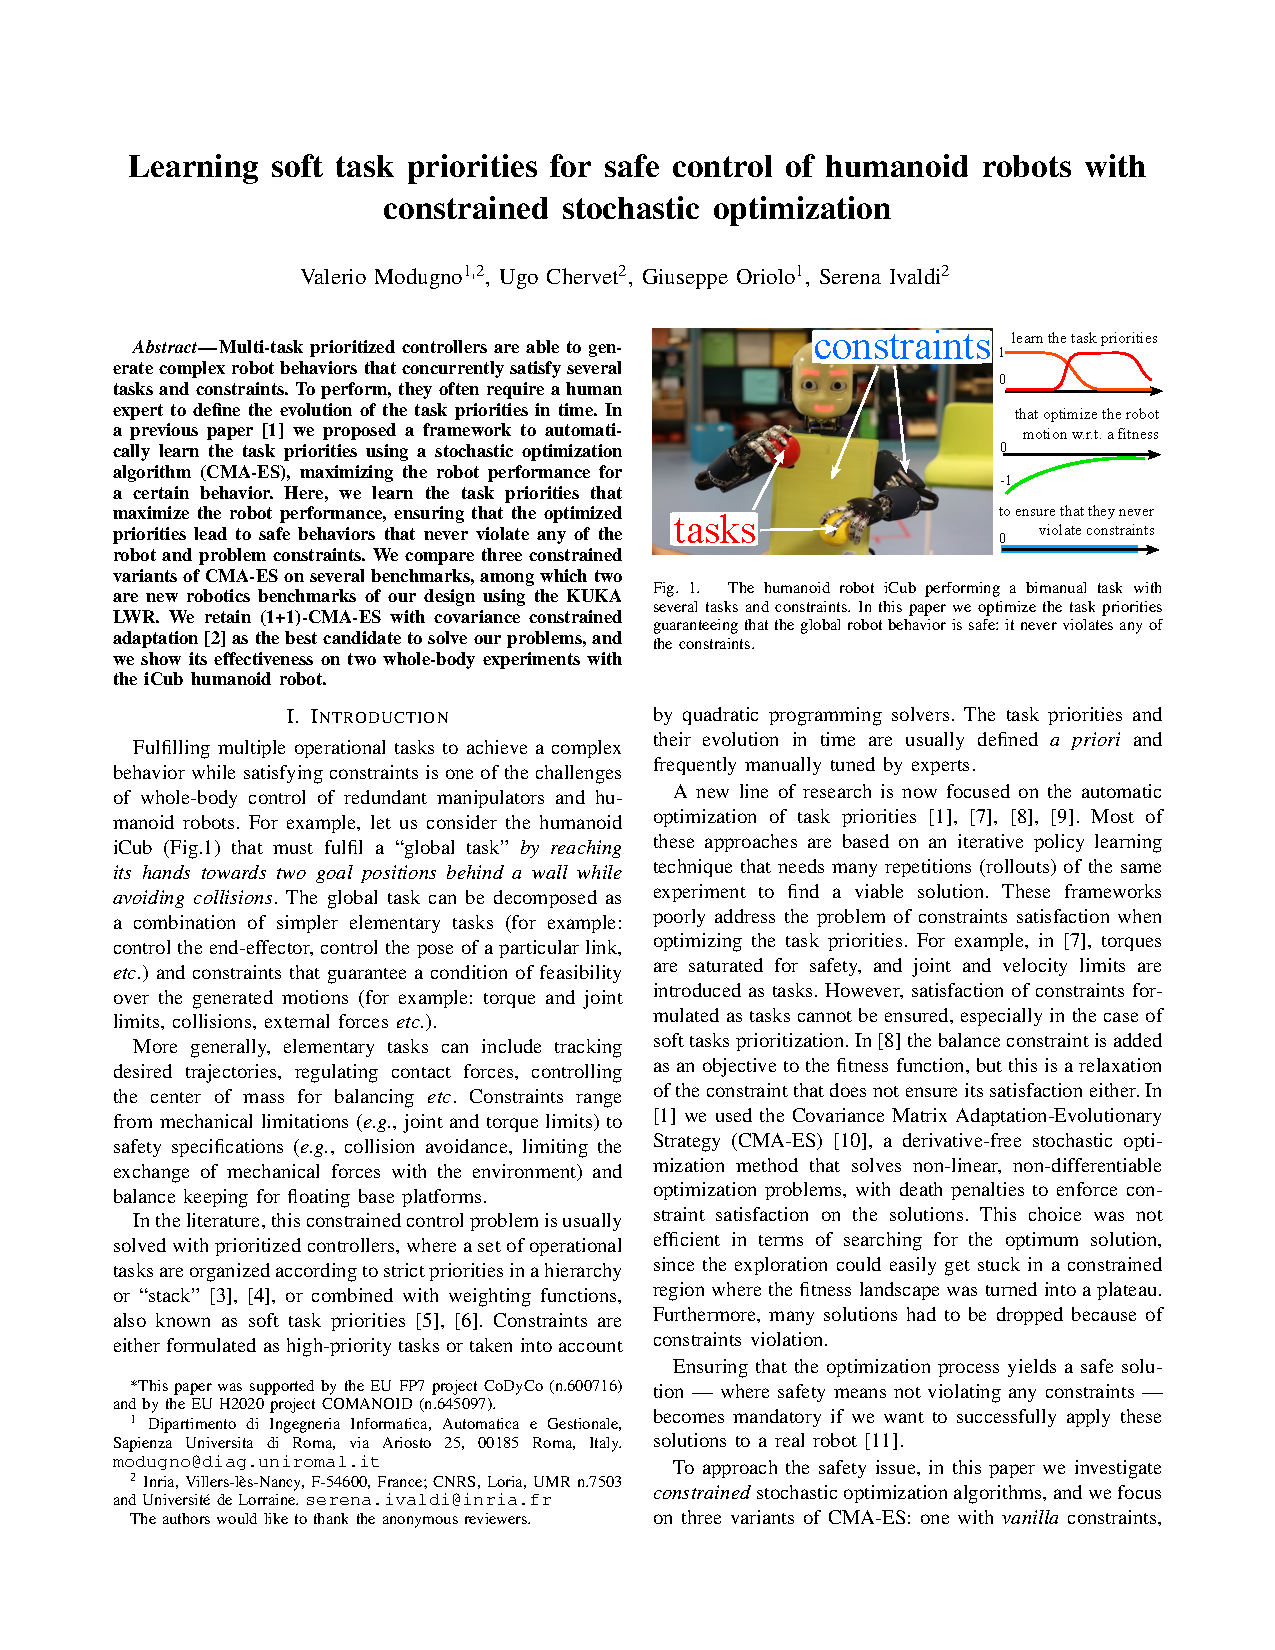
\includepdf[pages=-]{Modugno_HUMANOIDS_2016.pdf}

\chapter{Probabilistic Prioritization of Movement Primitives (TUDA)}\label{sec:Alex}
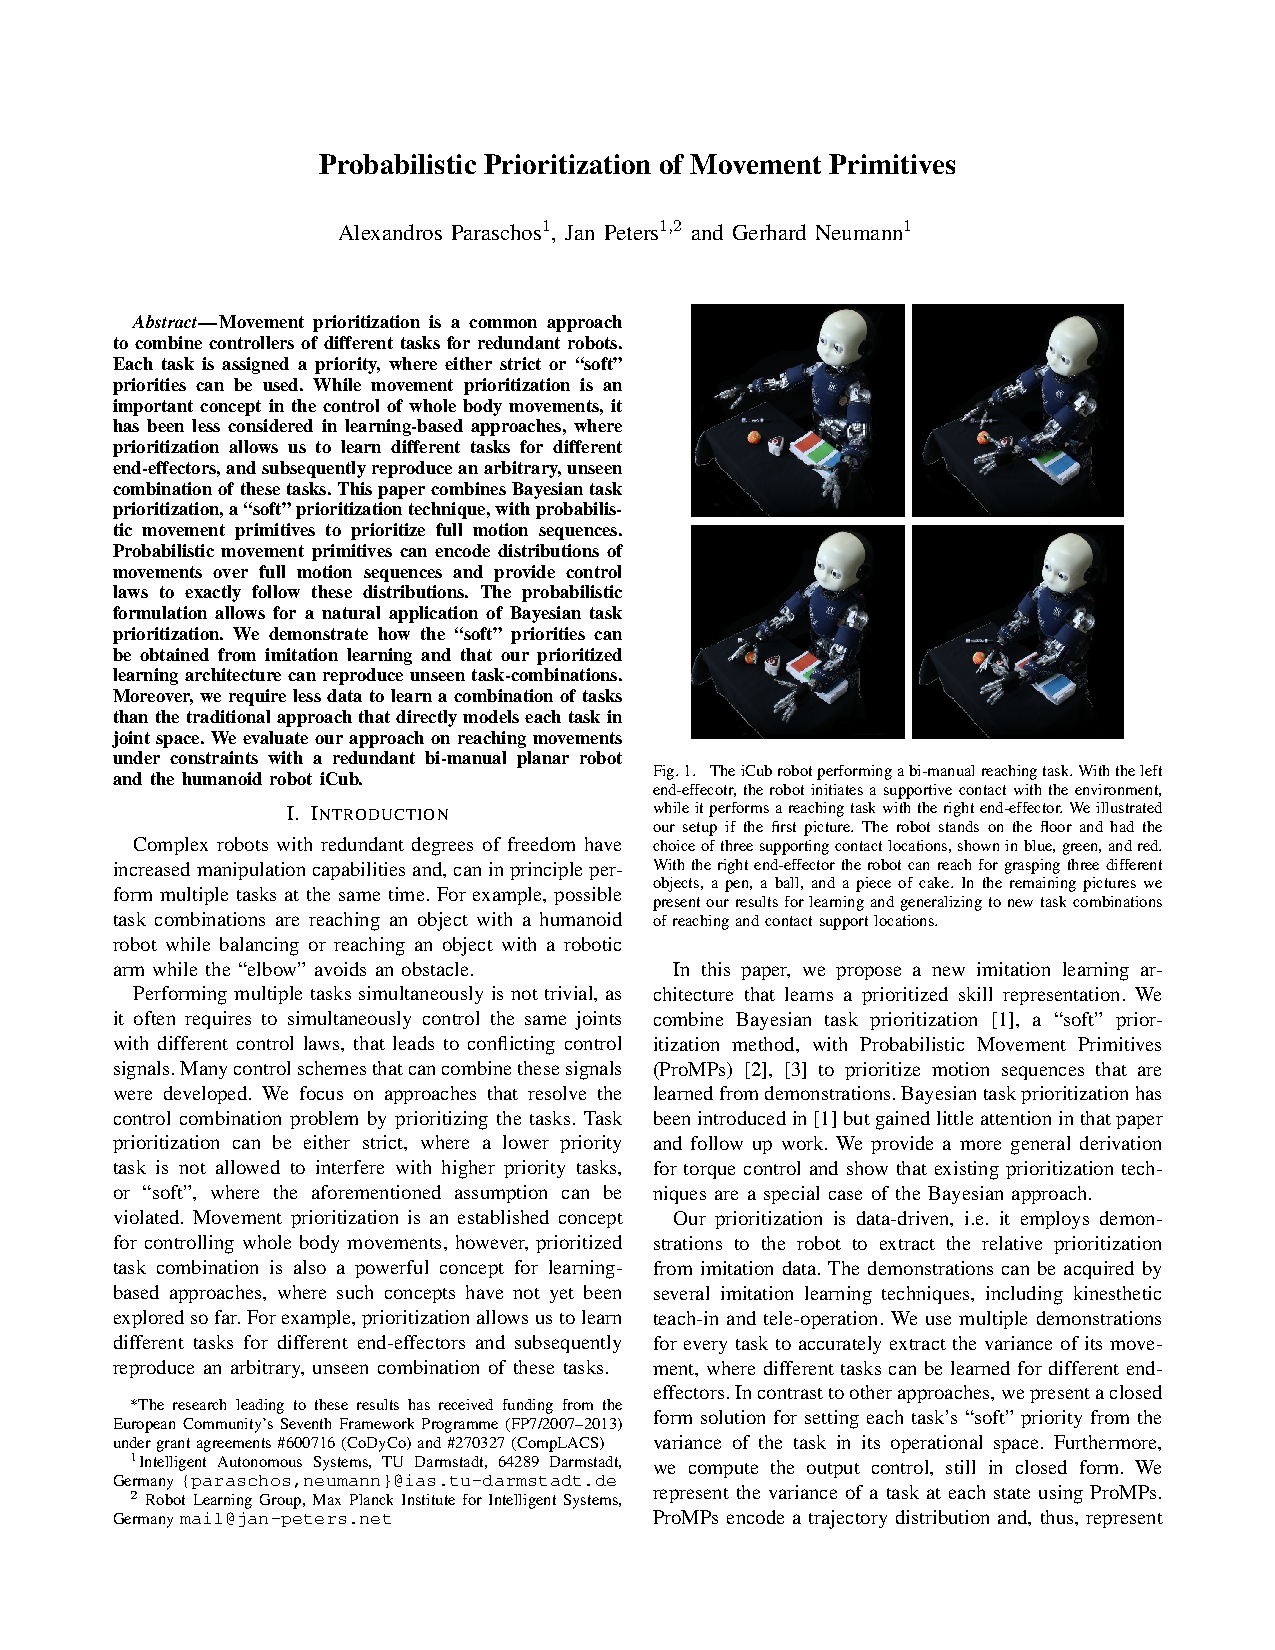
\includepdf[pages=-]{Paraschos_IROS_2017.pdf}

\bibliographystyle{plain}
\bibliography{manuscript}

\end{document}

%%% Local Variables:
%%% mode: latex
%%% TeX-master: t
%%% save-place: t
%%% End:
